\documentclass[11pt, oneside]{article}
\usepackage[utf8]{inputenc}
\usepackage{bm}
\usepackage{amsmath}
\usepackage{amsfonts}
\usepackage{amssymb}
\usepackage{graphicx}
\usepackage{ptex2tex, minted}
\usepackage{xcolor}
\usepackage{cancel}
\usepackage{caption}
\usepackage{subfigure}
\subfiglabelskip=0pt

\definecolor{gray}{gray}{0.97}
\colorlet{commentcolour}{green!50!black}
\colorlet{stringcolour}{red!60!black}
\colorlet{keywordcolour}{magenta!90!black}
\colorlet{exceptioncolour}{yellow!50!red}
\colorlet{commandcolour}{blue!60!black}
\colorlet{numpycolour}{blue!60!green}
\colorlet{literatecolour}{magenta!90!black}
\colorlet{promptcolour}{green!50!black}
\colorlet{specmethodcolour}{violet}
\colorlet{indendifiercolour}{green!70!white}

%\newcommand{\codetitlestyle}[1]{\small\textit{#1}\hspace{0.1cm}}
\newcommand{\belowtitleskip}{2pt}%\smallskipamount}
%\newcommand{\captionposition}{t}

%\newcommand{\mmo}[1]{\emph{#1}}

%\renewcommand{\ttdefault}{pcr}
\usepackage[T1]{fontenc}
\usepackage{lmodern}
\usepackage[top=3cm,bottom=4cm,left=3cm,right=3.2cm,asymmetric]{geometry}

\lstset{
numbers=none,
aboveskip=1ex,
belowskip=1ex,
basicstyle=\ttfamily\footnotesize,
}

\lstdefinestyle{pythonstyle}{
%%\lstset{
%%keepspaces=true,
language=python,
showtabs=true,
tab=,
tabsize=2,
basicstyle=\ttfamily\footnotesize,%\setstretch{.5},
stringstyle=\color{stringcolour},
showstringspaces=false,
alsoletter={1234567890},
otherkeywords={\ , \}, \{, \%, \&, \|},
keywordstyle=\color{keywordcolour}\bfseries,
emph={and,break,class,continue,def,yield,del,elif ,else,%
except,exec,finally,for,from,global,if,import,in,%
lambda,not,or,pass,print,raise,return,try,while,assert},
emphstyle=\color{blue}\bfseries,
emph={[2]True, False, None},
emphstyle=[2]\color{keywordcolour},
emph={[3]object,type,isinstance,copy,deepcopy,zip,enumerate,reversed,list,len,dict,tuple,xrange,append,execfile,real,imag,reduce,str,repr},
emphstyle=[3]\color{commandcolour},
emph={Exception,NameError,IndexError,SyntaxError,TypeError,ValueError,OverflowError,ZeroDivisionError},
emphstyle=\color{exceptioncolour}\bfseries,
%upquote=true,
morestring=[s]{"""}{"""},
morestring=[s]{'''}{'''},
commentstyle=\color{commentcolour}\slshape,
emph={[4]1, 2, 3, 4, 5, 6, 7, 8, 9, 0,ode, fsolve, sqrt, exp, sin, cos, arccos, pi, array, norm, solve,float,complex, dot, arange, isscalar, max, sum, flatten, shape, reshape, find, any, all, abs, plot, linspace, legend, quad, polyval,polyfit, hstack,vector, concatenate,vstack,column_stack,empty,zeros,ones,rand,vander,grid,pcolor,eig,eigs,eigvals,svd,qr,tan,det,logspace,roll,min,mean,cumsum,cumprod,diff,vectorize,lstsq,cla,eye,xlabel,ylabel,squeeze},
emphstyle=[4]\color{commandcolour},
emph={[5]__init__,__add__,__mul__,__div__,__sub__,__call__,__getitem__,__setitem__,__eq__,__ne__,__nonzero__,__rmul__,__radd__,__repr__,__str__,__get__,__truediv__,__pow__,__name__,__future__,__all__},
emphstyle=[5]\color{specmethodcolour},
emph={[6]assert,range,yield},
emphstyle=[6]\color{keywordcolour}\bfseries,
emph={[7]def, return, and, print},
emphstyle=[7]\color{black}\bfseries,
% emph={[7]self},
% emphstyle=[7]\bfseries,
literate=*%
%{:}{{\literatecolour:}}{1}%
%{=}{{\literatecolour=}}{1}%
%{-}{{\literatecolour-}}{1}%
%{+}{{\literatecolour+}}{1}%
%{*}{{\literatecolour*}}{1}%
{/}{{\literatecolour/}}{1}%
{!}{{\literatecolour!}}{1}%
%{(}{{\literatecolour(}}{1}%
%{)}{{\literatecolour)}}{1}%
%{[}{{\literatecolour[}}{1}%
%{]}{{\literatecolour]}}{1}%
{<}{{\literatecolour<}}{1}%
{>}{{\literatecolour>}}{1}%
{>>>}{{\textcolor{promptcolour}{>>>}}}{1}%
,%
breaklines=true,
breakatwhitespace= true,
xleftmargin=\framemargin,
xrightmargin=\framemargin,
aboveskip=1ex,
belowskip=1ex,
frame=trbl, %trbl
numbers=none,
%frameround=tttt,
rulecolor=\color{black!40},
%framexleftmargin=\framemargin,
%framextopmargin=.1ex,
%framexbottommargin=.1ex,
%framexrightmargin=\framemargin,
%framexleftmargin=1mm, framextopmargin=1mm, frame=shadowbox, rulesepcolor=\color{blue},#1
%frame=tb,
%backgroundcolor=\color{yellow!10}
backgroundcolor=\color{gray}
%}
}

\newcommand{\inpyth}{\lstinline[style=pythonstyle, basicstyle=\ttfamily]} %[]%

\lstnewenvironment{inpython}[1][]{
\lstset{style=pythonstyle, frame=trbl, belowcaptionskip=\belowtitleskip}
}{}

\newcommand{\includecode}[2][py]{\lstinputlisting[caption=#2,label=list:#2,style=pythonstyle,
float=!htpb]{#2}}

\newcommand{\hpl}[1]{({\bf hpl comment:} \emph{#1})}
\bibliographystyle{plain}

\title{Massively Parallel Python Implementation of a Pseudo-Spectral DNS Code for Turbulent Flow}
\author{Mikael Mortensen and Hans Petter Langtangen}
%\date{}							% Activate to display a given date or no date

\begin{document}
\maketitle
\section{Abstract}

\section{Introduction}
%\subsection{}
Direct Numerical Simulations (DNS) is a term reserved for computer simulations of turbulent flows that are fully resolved in both time and space. DNS are usually conducted using numerical methods of such high quality that numerical dispersion and diffusion errors are negligible compared to their actual physical counterparts. To this end, DNS has historically been carried out with extremely accurate and efficient spectral methods, and in the fluid dynamics community DNS enjoys  today the same status as carefully conducted experiments. DNS can provide detailed and highly reliable data not possible to extract from experiments, which in recent years have driven a number of discoveries regarding the very nature of turbulence. The present paper presents a new, computationally attractive tool for performing DNS, realized by recent programming technologies.

Because of the extremely heavy number crunching implied by DNS,
researchers aim at highly optimized implementations running on
massively parallel computing platforms. The largest known DNS
simulations performed today are using hundreds of billions of degrees
of freedom. Normally, this demands a need for developing tailored, hand-tuned
codes in what we here call low-level languages: Fortran, C, or C++. Few
DNS codes are openly available and easily accessible to the public and
the common fluid mechanics researcher. Some exceptions are hit-3d
(Fortran90) \cite{hit-3d}, Philofluid (Fortran) \cite{philofluid},
Tarang (C++) \cite{tarang}, and Turbo (Fortran90)
\cite{turbo}. However, the user interfaces to these codes are not highly developed and it is both challenging and time consuming for a user to to modify or extend the codes to satisfy their own needs. This is usually the nature of low-level codes.

It is a clear trend in computational sciences over the last two decades
that researchers tend to move from low-level languages to high-level languages
like Matlab, Python, R, and IDL. The experience is that implementations
in high-level languages are faster to develop, easier to test,
easier to maintain, and they
reach a much wider audience because the codes are compact and readable.
The downside has been the decreased computational
efficiency of high-level languages and in particular their lack of
suitability for massively parallel computing. In a field like computational
fluid dynamics, this argument has been a show stopper for wide use
of high-level languages. However, a language like Python has capabilities
today for providing short and quick implementations that compete with
tailored implementations in low-level languages up to thousands of processors.
This fact is not well known, and the purpose of this paper is to
demonstrate such a result for DNS and show the technical implementation
details that are needed.

%Because of the massive amounts of number crunching involved, DNS solvers are usually implemented in high entry-level, low-level languages like Fortran/Fortran90 or C/C++.

Python is a language that over the last two decades has grown very popular in the scientific computing community. A wide range of well established, ``gold standard'' scientific libraries in Fortran and C have been wrapped in Python, making them directly accessible just as commands in MATLAB. There is little overhead in calling low-level Fortran and C/C++functions from Python, and the computational speed obtained in a few lines of code may easily compete with hundreds of compiled lines of Fortran or C code. It is important new knowledge in the CFD community if flow codes can be developed with comfort and ease in Python without sacrificing much computational efficiency.

There are already several examples on successful use of Python for
high-performance parallel scientific computing. The sophisticated
finite element framework FEniCS \hpl{add ref!} is written mainly in
C++, but most application developers are writing FEniCS-based solvers
directly in Python, never actually finding themselves in need of
writing longer C++ code and firing up a compiler. For large scale
applications the devloped Python solvers are usually equally fast as
their C++ counterparts, because most of the computing time is usually
spent within the low-level wrapped C++ functions that perform the
costly linear algebra operations. \hpl{Should add parallel FEniCS numbers.}
GPAW \hpl{add ref!} is a code devoted
to electronic structure calculations, written as a combination of
Python and C. GPAW solvers written in Python have been shown to scale
well for thousands of processors.  The PETSc project is a major
provider of linear algebra to the open source community. PETSc was
developed in C, but through the package \texttt{petsc4py} almost all
routines may be set up and called from Python. PyClaw \hpl{add ref!}
is another good example, providing a compact, powerful, and intuitive
Python interface to the algorithms within the Fortran codes Clawpack
and SharpClaw. PyClaw is parallelised through PETSc and has been shown
to scale well up to 65,000 cores.

The ability of Python to wrap low-level, computationally highly efficient Fortran and C/C++ libraries for various applications is today well known, appreciated, and utilized by many. A lesser known fact is that basic Python modules like \texttt{numpy}, used for linear algebra and array manipulations, and \texttt{mpi4py}, which wraps (nearly) the entire MPI library, may be used directly to develop, from scratch, high performance solvers that run at speeds comparable to the very best implementations in low-level codes. A general misconception seems to be that Python may be used for fast prototyping and post-processing, as MATLAB, but that serious high-performance computing on parallel platforms require reimplementations in Fortran, C, or C++. In this paper, we conquer this misconception: The only real requirement for developing a fast pure \texttt{numpy}/\texttt{mpi4py} solver is that all array manipulations are performed using vectorization (that call underlying BLAS or LAPACK backends) such that explicit for loops over long arrays in Python are avoided. The \texttt{mpi4py} module in turn provides a message passing interface for \texttt{numpy} arrays at communication speeds very close to pure C code.

The major objective of this work is to explain a novel implementation of an excellent research tool for DNS, aimed at a wide audience. To this end, we i) show how a complete pseudo-spectral DNS solver can be written from scratch in Python using less than 100 lines of compact, very readable code, and ii) show that these 100 lines of code can run at speeds comparable to its low-level counterpart in hand-written C++ code. To establish scaling and benchmark results, we have run the codes on SHAHEEN, a massively parallel BlueGene/P machine at the KAUST Supercomputing Laboratory.

\section{Navier-Stokes in spectral space}
Our DNS implementation is based on a pseudo-spectral Galerkin method \cite{canuto1987} for the spatial discretization. The Navier-Stokes equations are first cast in rotational form

\begin{align}
 \frac{\partial \bm{u}}{\partial t} - \bm{u} \times \bm{\omega}   &= \nu \nabla^2 \bm{u} - \nabla{P}, \label{eq:NS} \\
 \nabla \cdot \bm{u} &= 0, \\
 \bm{u}(\bm{x}+2\pi \bm{e}^i, t) &= \bm{u}(\bm{x}, t), \quad \text{for }\, i=1,2,3,\\
 \bm{u}(\bm{x}, 0) &= \bm{u}_0(\bm{x})
\end{align}
where $\bm{u}(\bm{x}, t)$ is the velocity vector, $\bm{\omega}=\nabla \times \bm{u}$ the vorticity vector, $\bm{e}^i$ the Cartesian unit vectors, and the modified pressure $P=p+\bm{u}\cdot \bm{u}/2$, where $p$ is the regular pressure normalized by the constant density. The equations are periodic in all three spatial directions. If all three directions now are discretized uniformely in space using a structured computational mesh with $N$ points in each direction, the mesh points can be represented as
\begin{align}
{x}_j &= \frac{2\pi j}{N}, \quad j=0,\ldots, N-1,\\
\bm{x}^i_j &= x_j\bm{e}^i, \quad j=0,\ldots, N-1, \,\,i=1,2,3.
\label{eq:realmesh}
\end{align}
All variables may be transformed from the physical mesh $\bm{x}^i_j$ to a discrete and bounded Fourier wavenumber mesh using three-dimensional discrete Fourier transforms. Each point in the physical mesh will take part in three consecutive transformations, one for each periodic direction. The first transformed direction (arbitrary which one) is real and the remaining two are complex valued. There are in total $N^2$ real transforms of length $N$ and $2(N/2+1)N$ complex transforms of length $N$. The transforms in the three directions are performed sequentially. The first real transform along one line in the $z$-direction reads
\begin{align}
\mathcal{F}_{k_z}(\bm{u}) = \hat{\bm{u}}_{k_z}(t) &= \frac{2\pi}{N}\sum_{j=0}^{N-1}{\bm{u}({x}_j, t)}e^{-i k_z x_j}, \quad k_z=-N/2+1, \ldots, N/2,
\end{align}
with the inverse transform
\begin{align}
\mathcal{F}^{-1}_{j} (\hat{\bm{u}}) =\bm{u}(x_j, t) &= \frac{1}{2\pi}\sum_{k_z=-N/2+1}^{N/2}\hat{\bm{u}}_{k_z}(t)e^{i k_z {x}_j}, \quad j=0, \ldots, N-1.
\end{align}
Note that $i$ is used both as a spatial counter and as the imaginary unit. The
meaning should be clear from the context.

The transform is performed along all $N^2$ lines on the cubic mesh in the $z$-direction. To simplify notation, the complete three-dimensional transform for the entire mesh used in this work is denoted as
\begin{equation}
\mathcal{F}_{\bm{k}}(\bm{u}) = \hat{\bm{u}}_{\bm{k}}(t) = \mathcal{F}_{k_x}\left(\mathcal{F}_{k_y}\left(\mathcal{F}_{k_z}(\bm{u})\right)\right), \quad \bm{k}=(k_x, k_y, k_z).
\end{equation}
Note, however, that the order is arbitrary except from the data layout in memory. Similarily, using $i,j,k$ for the three Cartesian directions $x,y,z$, the inverse transform is defined as
\begin{equation}
\mathcal{F}^{-1}_{\bm{x}}(\hat{\bm{u}}) = \bm{u}(\bm{x}, t) = \mathcal{F}^{-1}_{k}\left(\mathcal{F}^{-1}_{j}\left(\mathcal{F}^{-1}_{i}(\hat{\bm{u}})\right)\right), \quad \bm{x} = (x, y, z),
\end{equation}
where the inverse transforms are taken in the opposite order of the forward transforms.

By taking the Fourier transform of the Navier-Stokes equations and subsequently the analythical spatial derivatives in spectral space, we obtain an ordinary differential equation for $\hat{\bm{u}}_{\bm{k}}$ and the continuity equation reduces to an orthogonal inner product
\begin{align}
 \frac{d\hat{\bm{u}}_{\bm{k}}}{d t} - \widehat{( \bm{u} \times \bm{\omega})}_{\bm{k}} &= - \nu |\bm{k}|^2  \hat{\bm{u}}_{\bm{k}} - i \bm{k} \hat{P}_{\bm{k}}, \label{eq:NSf} \\
 i \bm{k} \cdot \hat{\bm{u}}_{\bm{k}} &= 0.
\end{align}
The pressure may be eliminated by taking the divergence of (\ref{eq:NS}), or equivalently by dotting the transformed (\ref{eq:NSf}) by $i \bm{k}$ and rearranging such that
\begin{equation}
\hat{P}_{\bm{k}} = -i \frac{\bm{k} \cdot \widehat{( \bm{u} \times \bm{\omega})}_{\bm{k}} }{|\bm{k}|^2}.
\end{equation}
Inserting for the pressure in (\ref{eq:NSf}), the final equation to solve for each transformed velocity vector is thus
\begin{equation}
 \frac{d\hat{\bm{u}}_{\bm{k}}}{d t}  = \widehat{( \bm{u} \times \bm{\omega})}_{\bm{k}} - \nu |\bm{k}|^2  \hat{\bm{u}}_{\bm{k}} - \bm{k} \frac{\bm{k} \cdot \widehat{( \bm{u} \times \bm{\omega})}_{\bm{k}} }{|\bm{k}|^2}. \label{eq:NSfinal}
\end{equation}
Note that the transformed velocity components are coupled through the nonlinear convection term and the eliminated pressure.

The pseudo-spectral label arises from the treatment of the convective term, which is computed by first transforming the velocity and vorticity to physical space, performing the cross product, and then transforming the vector ${(\bm{u}  \times  \bm{\omega})}$  back to Fourier space. The operation requires 2 inverse transforms (velocity and vorticity) and 1 forward transform for each of the three vector components, 9 all together. Note that this is the only operation that requires MPI communication and it is typically the most computationally extensive part of a DNS solver.

The time integration of (\ref{eq:NSfinal}) is performed explicitly using a fourth order Runge-Kutta method, the Euler method or a second order Adams-Bashforth method. The details are left out here, but all algorithms simply need a function that returns the right hand side of (\ref{eq:NSfinal}).

\section{Implementation}

A Python solver for the pseudo-spectral Navier-Stokes equations is created in one main executable module. It is important to realize that the Python solver is not simply a wrapper of a low-level high-performance solver. Everything is implemented directly in Python - the mesh, the MPI domain decomposition and the Runge-Kutta integrator. We are only making use of wrappers for FFT, something that is also done by the majority of low-level solvers anyway. The current Python implementation may, as such, be used as a working prototype for a low-level implementation.

The solver makes use of the numpy and mpi4py packages that are imported in the very first part of the solver, see Fig. \ref{fig:preample}. Note that if the pyfftw module has been installed, it will be used to perform the FFT instead of numpy. Importing MPI from mpi4py initializes the MPI communicator. Two different strategies, slab and pencil, have been implemented for the MPI domain decomposition. However, since communication only enters through the FFTs there is very little difference between a serial code and a parallel. As such, we first present a serial version of the code.

\begin{figure}[t!]
\begin{python}
from numpy import *
from numpy.fft import fftfreq, fft, ifft, rfft, irfft
from mpi4py import MPI
comm = MPI.COMM_WORLD
num_processes = comm.Get_size()
rank = comm.Get_rank()
\end{python}
\caption{First lines of the solver are responsible for importing required functionality and for initializing the MPI communicator.}
\label{fig:preample}
\end{figure}


\subsection{Serial version of code}
The computational mesh is in physical space a structured uniform cube $[0, 2\pi]^3$, where each direction is divided into $N$ uniform intervals, where $N=2^M$ for $M\in \mathbb{Z}$. Any different size of the box may be trivially implemented through scaling. The mesh according to (\ref{eq:realmesh}) is implemented in Python as
\begin{python}
M = 6     # Assign the size of the mesh
N = 2**M  # Compute size of the mesh in each direction
X = mgrid[:N, :N, :N].astype(float)*L/N
\end{python}
where the matrix \inpyth{X} has dimensions \inpyth{X[3, N, N, N]}. Since the Navier Stokes equations are solved in Fourier space, the physical space is only used to compute the convection plus to do postprocessing. The mesh \inpyth{X} is typically used for initialization and otherwise not needed. As such, it may be deleted to save memory. In parallel mode, \inpyth{X} will be split up and divided between the processors.  Note that the solver may be operated in either single or double precision mode, and that \inpyth{float} is a placeholder for either one of the \inpyth{numpy} datatypes \inpyth{float32} or \inpyth{float64}, depending on settings.

The velocity field to be transformed is real, and the discrete Fourier transform of a real sequence has the property that $\hat{\bm{u}}_k = \hat{\bm{u}}_{N-k}^*$, where $^*$ denotes the complex conjugate. As such, it is sufficient to use $N/2+1$ Fourier coefficients, leading to a transformed wavenumber mesh of size $(N/2+1)N^2$. The highest frequency (the Nyquist frequency $k=N/2+1$) is often neglected in turbulence simulations because "this is a coefficient for a Fourier mode that is not carried in the
Fourier representation of the solution" \cite{Lee2013}. For the MPI slab decomposition the Nyquist frequency is included, whereas it is neglected for the 2D pencil decomposition. For MPI communication reasons, the real transform is taken in the final z direction and the wavenumbers $\bm{k}=(k_x, k_y, k_z)$ stored on the transformed mesh thus has ordering as used by the FFT routines provided by numpy (and pyfftw)
\begin{align}
  \bm{k} = [&(0, \ldots, N/2-1, -N/2, -N/2+1, \ldots, -1), \notag \\
   &(0, \ldots, N/2-1, -N/2, -N/2+1, \ldots, -1),  \notag \\
  &(0, \ldots, N/2-1, N/2)].
\end{align}
The wavenumber mesh is implemented as
\begin{python}
Nf = N/2+1
kx = ky = fftfreq(N, 1./N).astype(int)
kz = kx[:Nf].copy(); kz[-1] *= -1
KX = array(meshgrid(kx, ky, kz, indexing='ij'), dtype=int)
KK = sum(KX*KX, 0, dtype=int)
KX_over_Ksq = KX.astype(float) / where(KK==0, 1, KK).astype(float)
\end{python}
where \inpyth{fftfreq(N, 1./N)} is a function that creates the wavenumbers $(0, \ldots, N/2-1, -N/2, -N/2+1, \ldots, -1)$. The dimesions of the matrices are \inpyth{KX[3, N, N/2+1, N]}, \inpyth{KK[N, N/2+1, N]} and \inpyth{KX_over_Ksq[3, N, N/2+1, N]}, and the matrices represent $\bm{k}$, $|\bm{k}|^2$ and $\bm{k}/|\bm{k}|^2$ respectively. The last two matrices are precomputed for efficiency.

The velocity, curl and pressure are similarily stored in structured numpy arrays
\begin{python}
U     = empty((3, N, N, N), dtype=float)
U_hat = empty((3, N, N, Nf), dtype=complex)
P     = empty((N, N, N), dtype=float)
P_hat = empty((N, N, Nf), dtype=complex)
curl  = empty((3, N, N, N))
\end{python}
Here \inpyth{hat} represents a transformed variable. To tranform between, e.g., \inpyth{U} and \inpyth{U_hat}, calls to FFT routines are required. The three dimensional FFT and its inverse are implemended in Python functions as shown below.

\begin{python}
def fftn_mpi(u, fu):
    """FFT of u in three directions."""
    if num_processes == 1:                # Scalar version
        fu[:] = rfftn(u, axes=(0,1,2))
    return fu

def ifftn_mpi(fu, u):
    """Inverse FFT of fu in three directions."""
    if num_processes == 1:                # Scalar version
        u[:] = irfftn(fu, axes=(0,1,2))
    return u

# Usage
U_hat = fftn_mpi(U, U_hat)
U = ifftn_mpi(U_hat, U)
\end{python}
For high performance, it is key that the Python code relies on \emph{in-place}
modifications of pre-allocated arrays to avoid unnecessary allocation of
large temporary arrays (which often arises from basic \texttt{numpy} code).
Each of the functions above takes the result array (\texttt{U\_hat} or
\texttt{U}) as argument, fill this array with values and returns the
array to the calling code. A commonly applied convention in
Python is to return all result objects from functions as this only involves
transfer of references and no copying of data.

We also remark that the three consecutive transforms performed by \inpyth{rfftn/irfftn} are actually using one real transform along the $y$-direction and two complex transforms in the remaining two directions. Also note that the simple [[[numpy/pyfftw wrapped functions \inpyth{rfftn/irfftn} may only be used in single processor mode and the MPI implementation is detailed in Sec ?.

The convection term requires a transform from Fourier to physical space where the cross product $\bm{u} \times \bm{\omega}$ is carried out. The curl in Fourier space is
\begin{equation}
\mathcal{F}_{\bm{k}}(\nabla \times \bm{u}) = \hat{\bm{\omega}}_{\bm{k}} = i \bm{k} \times \hat{\bm{u}}_{\bm{k}}.
\end{equation}
We can now compute the curl in physical space through $\bm{\omega} = \mathcal{F}_{\bm{x}}^{-1}(\hat{\bm{\omega}})$. The convection term may thus be computed as
\begin{equation}
\widehat{( \bm{u} \times \bm{\omega})}_{\bm{k}} = \mathcal{F}_{\bm{k}}(\bm{u} \times \bm{\omega}) = \mathcal{F}_{\bm{k}} (\mathcal{F}^{-1}_{\bm{x}}(\hat{\bm{u}}) \times \mathcal{F}^{-1}_{\bm{x}}(\hat{\bm{\omega}})).
\end{equation}
where the implemented functions to do the curl and cross products are
\begin{python}
def Cross(a, b, c):
    """c = F(a x b)"""
    fftn_mpi(a[1]*b[2]-a[2]*b[1], c[0])
    fftn_mpi(a[2]*b[0]-a[0]*b[2], c[1])
    fftn_mpi(a[0]*b[1]-a[1]*b[0], c[2])

def Curl(a, c):
    """c = F_inv(curl(a))"""
    ifftn_mpi(1j*(KX[0]*a[1]-KX[1]*a[0]), c[2])
    ifftn_mpi(1j*(KX[2]*a[0]-KX[0]*a[2]), c[1])
    ifftn_mpi(1j*(KX[1]*a[2]-KX[2]*a[1]), c[0])

\end{python}
The entire right hand side of (\ref{eq:NSfinal}) is implemented as shown in Fig. \ref{fig:computeRHS}. The convection term is dealiased using the 2/3-rule and dealiasing is simply achieved by an elementwise multiplication of the convection matrix \inpyth{dU[3, N, N/2+1, N]} with matrix \inpyth{dealias[N, N/2+1, N]}, that is zero where the wavenumbers are larger than 2/3 of the Nyquist mode and one otherwise. Note that the dimensions of \inpyth{dU} and \inpyth{dealias} differ in the first index since \inpyth{dU} contains contributions for all three vector components. However, through automatic broadcasting numpy realizes that the last three dimensions are the same and as such all three components of \inpyth{dU} (i.e.,  \inpyth{dU[0]}, \inpyth{dU[1]} and  \inpyth{dU[2]}) are multiplied elementwise with the same matrix \inpyth{dealias}. The parameters \inpyth{nu} and \inpyth{dt} are the viscosity and time step respectively and they are both declared as global variables in the beginning of the solver. The advancement in time can be performed in its simplest possible form through the Forward Euler method as shown in Fig. \ref{fig:FEuler}.
\begin{figure}[h!]
\begin{python}
# Declare some matrices and parameters
kmax = N/3.
dU = empty((3, N, Nf, N), dtype=complex)
dealias = array((abs(KX[0]) < kmax)*(abs(KX[1]) < kmax)*
                (abs(KX[2]) < kmax), dtype=bool)
dt = 0.01    # Time step
nu = 0.001   # Viscosity

def ComputeRHS(dU, rk):
    if rk > 0: # For rk=0 the correct values are already in U
        for i in range(3):
            ifftn_mpi(U_hat[i], U[i])

    # Compute convective term and place in dU
    Curl(U_hat, curl)
    Cross(U, curl, dU)

    # Dealias the nonlinear convection
    dU[:] *= dealias*dt

    # Compute pressure (To get actual pressure multiply by 1j/dt)
    P_hat[:] = sum(dU*KX_over_Ksq, 0)

    # Add pressure gradient
    dU[:] -= P_hat*KX

    # Add contribution from diffusion
    dU[:] -= nu*dt*KK*U_hat

\end{python}
\caption{Function for computing the right hand side of Eq. (\ref{eq:NSfinal}).}
\label{fig:computeRHS}
\end{figure}

\begin{figure}
\begin{python}
t = 0        # Actual time
T = 1.0      # End time
while t < T-1e-8:
    t += dt
    tstep += 1
    ComputeRHS(dU, 0)
    U_hat[:] += dU
\end{python}
\caption{Forward Euler method for time advancement of Eq. (\ref{eq:NSfinal}).}
\label{fig:FEuler}
\end{figure}

\subsection{1D Slab decomposition}
To run the code on several processors using MPI, the data structures need to be split up. In the litterature the most popular strategy is "slab" decomposition, where each CPU is assigned responsibility for a certain number of complete 2D planes (slices). In other words, just one of the three indices $(i,j,k)$ is split up and divided amongst the CPUs. The major drawback of the slab decomposition strategy is that the number of CPUs must be smaller than or equal to $N$ for a cubic mesh of size $N^3$.

The meshes for the slab decomposition are implemented as shown in Fig. \ref{fig:1Dslabmesh}. In general, using \inpyth{num_processes} CPUs, each CPU gets responsibility for \inpyth{Np = N/num_processes} slices and the physical mesh is simply decomposed along the first index. The wavenumber mesh, on the other hand, is split along the third direction. The reason for this choice is that the $k_x$ direction is the last direction to be transformed by the three consecutive FFTs (see Fig. \ref{fig:serialfft}) and for this operation the data structures need to be aligned in the $k_x$ direction.
\begin{figure}
\begin{python}
Np = N / num_processes
X = array(meshgrid(x[rank*Np:(rank+1)*Np], x, x, indexing='ij'))
KX = array(meshgrid(kx, ky, kz[rank*Np:(rank+1)*Np], indexing='ij'), dtype=int)
\end{python}
\caption{1D slab decomposition of physical mesh and wavenumber mesh.}
\label{fig:1Dslabmesh}
\end{figure}

The MPI decomposition is easily understood by the illustrations in Fig. \ref{fig:Slabdecomp}, which is using 4 CPUs for a physical mesh of size $8^3$. Each processor does a complete two dimensional FFT in both y and z directions on the original real data structure. To do the final transform in the $x$-direction, data must be communicated between all processors. The communication takes place in one single \inpyth{MPI Alltoall} operation and one transform from the data structure in Fig \ref{subfig1} to the one in \ref{subfig2}. The entire 3D parallel FFT may be implemented with 5 lines of Python code as shown in Fig \ref{fig:slabfft}. Note that  \inpyth{Alltoall} requires two work arrays as placeholders, one for each of the data structures seen in Fig \ref{fig:Slabdecomp} (b) and (c). Alternatively, the data transfer may be performed without explicit work arrays using the in-place \inpyth{Sendrecv_replace} along with transpose operations, as shown in the commented code in Fig \ref{fig:slabfft_sendrecv}.
\begin{figure}[t!]
\subfigure[Physical mesh]{
  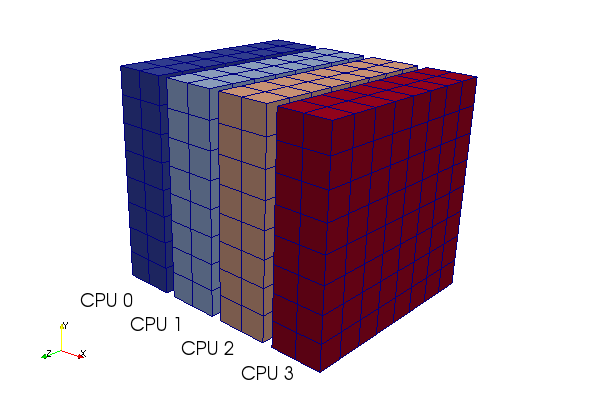
\includegraphics[scale=0.4]{SlabReal.png}
  \label{subfig0}
  }
\subfigure[Wavenumber mesh after real transform]{
  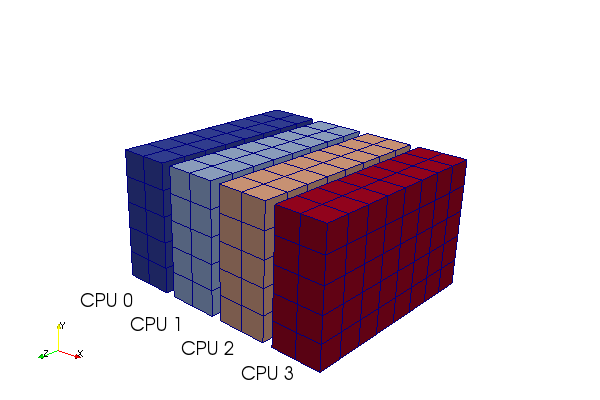
\includegraphics[scale=0.4]{SlabReal2.png}
  \label{subfig1}
}
\subfigure[Final wavenumber mesh.]{
  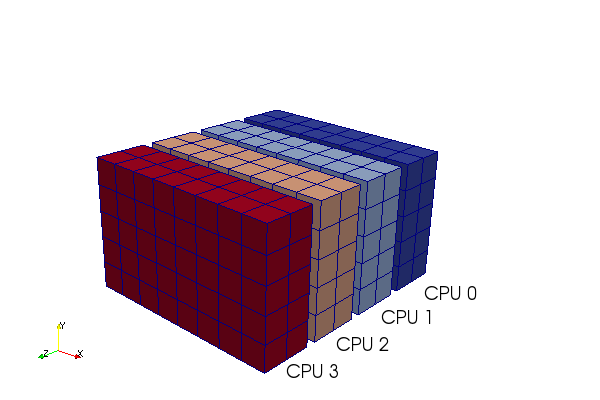
\includegraphics[scale=0.4]{SlabComplex.png}
  \label{subfig2}
  }
\caption{Slab decomposition of physical \subref{subfig0} and wavenumber meshes \subref{subfig1}, \subref{subfig2}. }
\label{fig:Slabdecomp}
\end{figure}

\begin{figure}
\begin{python}
def fftn_mpi(u, fu):
    """fft in three directions using mpi
    """
    Uc_hatT[:] = rfft2(u, axes=(2,1))
    for i in range(num_processes):
        U_mpi[i] = Uc_hatT[:, :, i*Np:(i+1)*Np]
    comm.Alltoall([U_mpi, MPI.DOUBLE_COMPLEX], [fu, MPI.DOUBLE_COMPLEX])
    fu[:] = fft(fu, axis=0)

def ifftn_mpi(fu, u):
    """ifft in three directions using mpi.
    Need to do ifft in reversed order of fft
    """
    Uc_hat[:] = ifft(fu, axis=0)
    comm.Alltoall([Uc_hat, mpitype], [U_mpi, mpitype])
    for i in range(num_processes):
        Uc_hatT[:, :, i*Np:(i+1)*Np] = U_mpi[i]
    u[:] = irfft2(Uc_hatT, axes=(2,1))

\end{python}
\caption{Three dimensional parallel FFT and inverse FFT with slab decomposition. Three intermediate complex work arrays \inpyth{Uc_hatT[Np, N/2+1, N]}, \inpyth{Uc_hatT[N, N/2+1, Np]} and \inpyth{Uc_mpi[N, N/2+1, Np]} are used.}
\label{fig:slabfft}
\end{figure}

\subsection{2D Pencil decomposition}
For massively parallel simulations the slab decomposition falls short since the number of CPUs allowed is limited by $N$, where the size of the physical box is $N^3$. For large scale simulations using up to $N^2$ CPUs, the 2D pencil decomposition, first suggested by Ding, Ferraro and Gennery in 1995 \cite{Ding95}, is commonly used. Publically available implementations of the 3D parallel FFT that makes use of the pencil decomposition are the Parallel FFT Subroutine Library by \cite{PlimptonFFT}, the P3DFFT library by Pekurovsky \cite{p3dfft, Pekurovsky2012}, the 2DECOMP\&FFT library by Li and Laizet \cite{Li2010} and PFFT by Pippig \cite{Pi13}.

The 2D pencil decomposition strategy is illustrated in Fig. \ref{fig:Pencildecomp} for a box of size $16^3$, using 4 CPUs. The datastructures are split in the plane normal to the direction where we are performing the 1D FFTs. That is, for the physical mesh in Fig. \ref{fig:Pencildecomp} (a) the $x-z$ plane is split up in a $2\times2$ processor mesh. Each CPU may now perform 64 ($= 8 \times 8$) 1D real FFTs in the $y$-direction on its $8 \times 8 \times 16$ physical mesh. Afterwords, the complex data will be laid out as shown in Fig. \ref{fig:Pencildecomp} (b). The second transform will take place in the $x$-direction and for this to happen data must be exchanged between processors 0 and 1 as well as 2 and 3. The datastructures must also be transposed to the shape seen in Fig. \ref{fig:Pencildecomp} (c). Each CPU may now perform the 32 ($4 \times 8$) individual 1D FFTs in the $x$-direction. The same procedure is followed to end up with datastructures aligned in the final $z$-direction, see Fig. \ref{fig:Pencildecomp} (d). However, this time processor 0 communicates with processor 2 and likewise 1 with 3.

Evidently, each processor belongs to two different groups of communicators. One for communication in the $x-y$ plane (Fig. \ref{fig:Pencildecomp} (b) to (c)) and one for communication in the $x-z$ plane (Fig \ref{fig:Pencildecomp} (c) to (d)). The MPI communicator groups and the distributed mesh are created in Python as shown in Fig. \ref{fig:commgroups}.

\begin{figure}
\subfigure[Physical mesh]{
  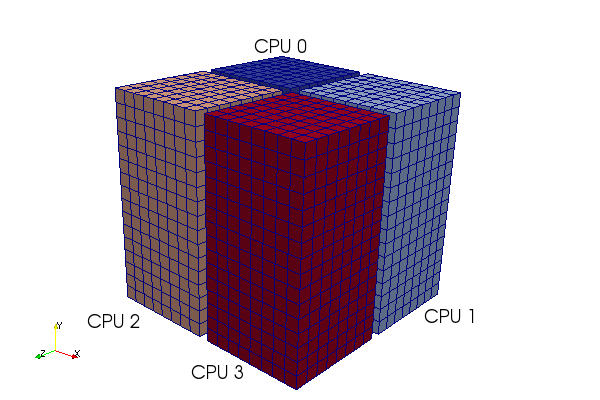
\includegraphics[scale=0.44]{Pencil1.png}
  \label{subfig0}
  }
\subfigure[Wavenumber mesh after real transform]{
  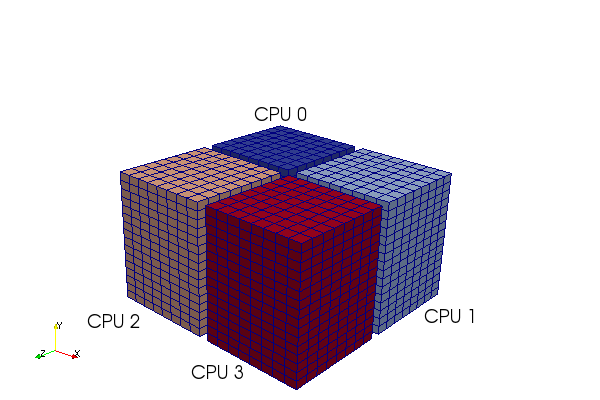
\includegraphics[scale=0.44]{Pencil2.png}
  \label{subfig1}
}
\subfigure[Intermediate wavenumber mesh]{
  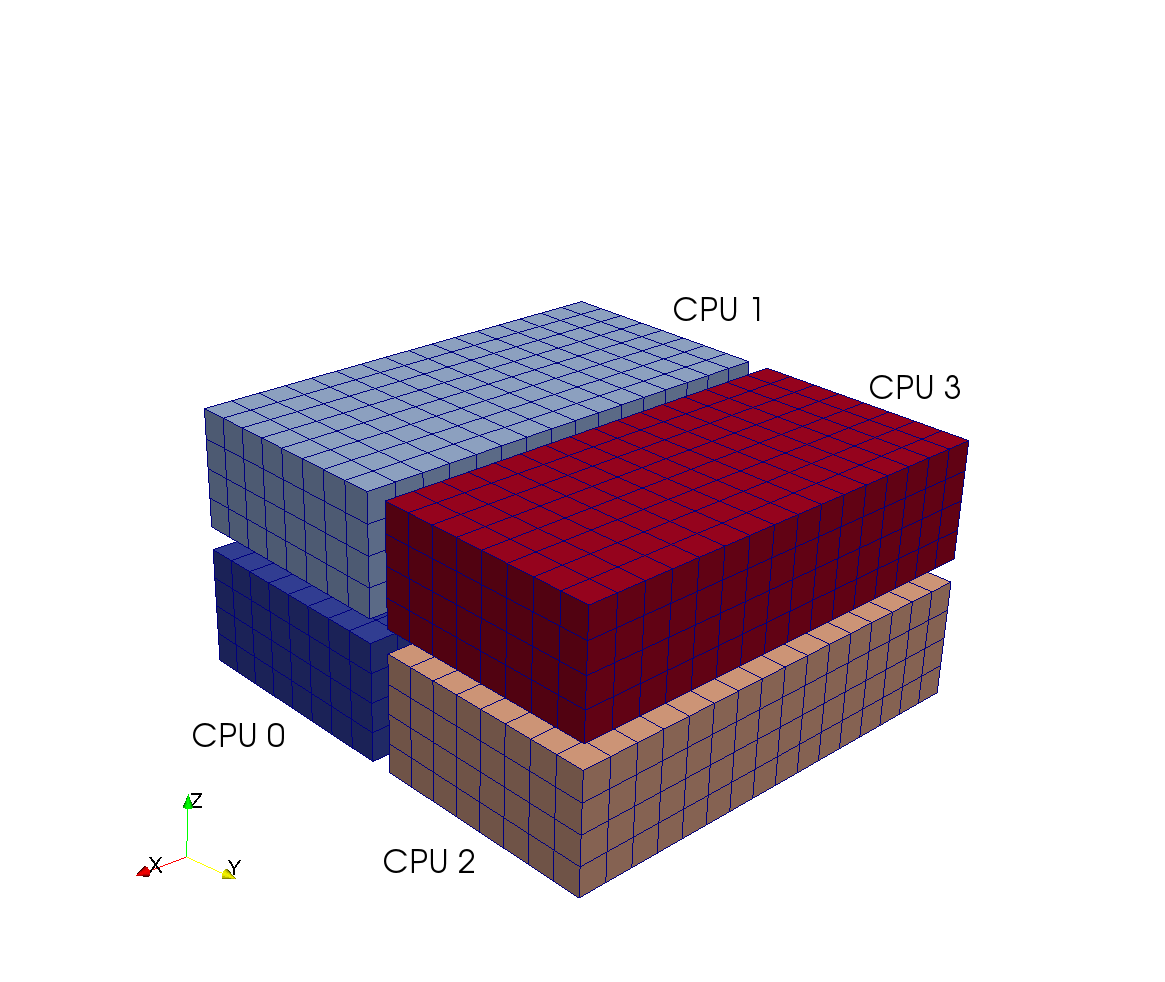
\includegraphics[scale=0.44]{Pencil3.png}
  \label{subfig2}
  }
\subfigure[Final wavenumber mesh.]{
  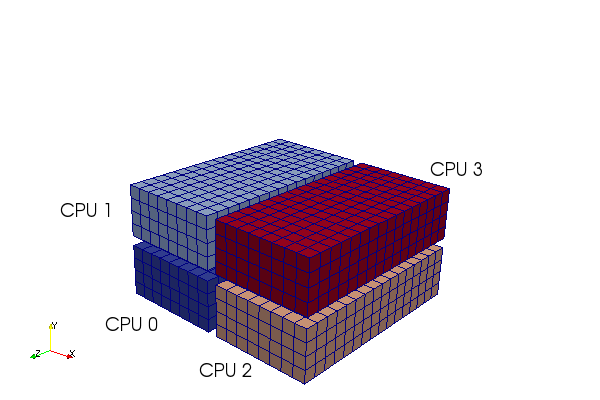
\includegraphics[scale=0.44]{Pencil4.png}
  \label{subfig3}
  }
\caption{2D pencil decomposition of physical mesh \subref{subfig0} and the three wavenumber meshes \subref{subfig1}, \subref{subfig2}, \subref{subfig3}. The decomposition shown uses 4 CPUs, two in each direction normal to the direction of the current one-dimensional FFT. The FFT in the y-direction transforms data in \subref{subfig0} to \subref{subfig1}. The data is then transformed and communicated to the composition seen in \subref{subfig2}. Here the FFT in $x$-direction is carried out before the data is transformed again and communicated to \subref{subfig3}, where the final FFT is performed.}
\label{fig:Pencildecomp}
\end{figure}

\begin{figure}
\begin{python}
num_processes = comm.Get_size() # Total number of CPUs
rank = comm.Get_rank()  # Global rank
P1 = 2     # Assign number of CPUs in first direction
P2 = num_processes / P1 # CPUs in second direction
N1 = N/P1
N2 = N/P2

# Create two communicator groups for each rank
commxz = comm.Split(rank%P1)
commxy = comm.Split(rank/P1)

xyrank = commxy.Get_rank() # Local rank in xy-plane
xzrank = commxz.Get_rank() # Local rank in xz-plane

# Create the physical mesh
x = linspace(0, L, N+1).astype(float)[:-1]
x1 = slice(xyrank * N1, (xyrank+1) * N1, 1)
x2 = slice(xzrank * N2, (xzrank+1) * N2, 1)
X = array(meshgrid(x[x1], x, x[x2], indexing='ij'), dtype=float)
\end{python}
\caption{Creation of two MPI communicator groups, \inpyth{commxy} and \inpyth{commxz}, and the decomposed physical mesh \inpyth{X[3, N1, N, N2]}. With reference to Fig. \ref{fig:Pencildecomp}, the two communicator groups for CPU with global rank 0 is \inpyth{commxy} = [0, 1] and \inpyth{commxz} = [0, 2].}
\label{fig:commgroups}
\end{figure}

The entire 9 lines of code for the Python implementation of the 3D parallel FFT is shown in Fig. \ref{fig:fftn_mpi_pencil}. Note that data communication is performed when the data are aligned with the $x$-direction (Fig. \ref{fig:Pencildecomp} (c)). Here the datastructure is of shape \inpyth{Uc_hat_x[N, N1/2, N2]}, where \inpyth{N1=N/P0} and \inpyth{N2=N/P1} and \inpyth{P0} and \inpyth{P1} are the division of processors used for the two split directions. In Fig. \ref{fig:Pencildecomp} \inpyth{P0} = \inpyth{P1} = 2. In the call to \inpyth{Alltoall} the first dimension of \inpyth{Uc_hat_x}, i.e. $N$, is automatically broadcasted such that \inpyth{Uc_hat_x[P1, N1, N1/2, N2]}

\begin{figure}
\begin{python}
def fftn_mpi(u, fu):
    """Three dimensional fft using mpi
    """
    # Do fft in y direction on owned real data u
    Uc_hat_y[:] = rfft(u, axis=1)

    # Transform to x direction neglecting Nyquist mode
    for i in range(P1):
        Uc_hat_x[i*N1:(i+1)*N1] = Uc_hat_y[:, i*N1/2:(i+1)*N1/2]

    # Communicate and do fft in x-direction
    commxy.Alltoall([Uc_hat_x, mpitype], [Uc_hat_xr, mpitype])
    Uc_hat_x[:] = fft(Uc_hat_xr, axis=0)

    # Communicate and transform to final z-direction
    commxz.Alltoall([Uc_hat_x, mpitype], [Uc_hat_xr, mpitype])
    for i in range(P2):
        Uc_hat_z[:, :, i*N2:(i+1)*N2] = Uc_hat_xr[i*N2:(i+1)*N2]

    # Do fft for last direction
    fu[:] = fft(Uc_hat_z, axis=2)

\end{python}
\caption{Three dimensional FFT with pencil decomposition. The work arrays \inpyth{Uc_hat_y, Uc_hat_x, Uc_hat_z} are laid out as seen in Fig. \ref{fig:Pencildecomp} (b), (c) and (d) respectively. The array \inpyth{Uc_hat_xr} is a copy of \inpyth{Uc_hat_x} used only for communication.}
\label{fig:fftn_mpi_pencil}
\end{figure}


\appendix

\begin{figure}
\begin{python}
def fftn_mpi(u, fu):
    """fft in three directions using mpi
    Alternative MPI-implementation
    """
    # Do FFT for two directions, first real
    ft = fu.transpose(2,1,0)
    ft[:] = rfft2(u, axes=(2,1))

    # Create transformed view of fu array
    fu_send = fu.reshape((num_processes, Np, Nf, Np))

    # Communicate
    for i in range(num_processes):
        if not i == rank:
            comm.Sendrecv_replace([fu_send[i], MPI.DOUBLE_COMPLEX], i, 0, i, 0)

    # Align data with final x-direction
    fu_send[:] = fu_send.transpose(0,3,2,1)

    # Do fft for last direction
    fu[:] = fft(fu, axis=0)

def ifftn_mpi(fu, u):
    """ifft in three directions using mpi.
    Alternative MPI-implementation
    """
    # Do inverse FFT of first owned direction
    Uc_hat[:] = ifft(fu, axis=0)

    # Create transformed view of Uc_hat
    Uc_send = Uc_hat.reshape((num_processes, Np, Nf, Np))

    # Communicate and transform
    for i in range(num_processes):
       if not i == rank:
           comm.Sendrecv_replace([Uc_send[i], MPI.DOUBLE_COMPLEX], i, 0, i, 0)
       Uc_hatT[:, :, i*Np:(i+1)*Np] = Uc_send[i]

    # Do inverse FFT for last two directions, final real
    u[:] = irfft2(Uc_hatT, axes=(2,1))

\end{python}
\caption{Three dimensional parallel FFT with slab decomposition. Note that no explicit work arrays are used with the forward transform.}
\label{fig:slabfft_sendrecv}
\end{figure}

\bibliography{bib.bib}


\end{document}
